%!TEX root = ../../../../report.tex

\subsection{The electric actuators} % (fold)
\label{sub:electric_actuators}
In chapter \ref{cha:mathematical_model}, the necessary characteristics of the actuators have been calculated.
In this section, the resulting theoretical requirements are used to select the final motor $+$ gearbox combination utilized.
All the documentation regarding the control of the actuators software-wise is to be found in section \ref{sec:software}.

\subsubsection{Flat BLDC Maxon motors} % (fold)
\label{ssub:the_bldc_motors}
It must be mentioned at this point that the actuators and their interface were assumed at the beginning of the project to be a very hard constraint in the design from an economic point of view. 
This means that the conception of the robot structure has been influenced by this criteria towards the adaption of the final prototype characteristics (such as final size or mass) to the application range of the available motors at our disposal.
This fact has converted the design in an iterative process of optimization whose final result is a robot that matches the available actuators and not the other way around, as it should be in theory.
In the view of the this, the brushless DC motor $+$ gearbox present in the Locokit robot construction kit, introduced in \cite{locokit} are used in the Rubi prototype.

The flat motors model is 339260 from Maxon motor, whose datasheet can be found in \cite{maxon_motor}, and the planetary gearhead is the number 143976 in datasheet \cite{maxon_gear}.
The electromechanical constants of the motors, together with its nominal supply values or the output power and torque of both the motor and the gearbox can be found in these documents. 
However, the electronics of the motors is designed to constantly overdrive them at $24V$, which has been taken into account when calculating their output.
Furthermore, each motor counts three hall effect sensors able to provide accurate relative position measurements.

% subsubsection the_bldc_motors (end)


\subsubsection{BLDC motor boards} % (fold)
\label{ssub:bldc_motor_boards}
Each BLDC motor in the Locokit comes with a motor board able to control it, designed for 24V and 48W.
They consist of a 48MHz ARM7 processor for time critical control and motor commutation, as stated in \cite{locokit-electronics}, together with 4 general purpose I/O inputs for local sensor interface.
Furthermore, they have two available 8-pin interfaces for the motors, one of them with a standard flex connector used in most of Maxon flat motors.

% subsubsection bldc_motor_boards (end)

\subsubsection{Extension PCBs} % (fold)
\label{ssub:extension_pcbs}
Following the idea of reducing weight and inertias in the structure as explained in chapter \ref{cha:analysis}, it was decided to place all the electronics off-board.
In order to extended the existing motor flex interfaces, a simple extension PCB was manufactures for each device.
The board for the left leg, whose schematic can be seen in \ref{fig:pcb1} \footnote{For the right leg the schematic has been mirrored}, contains a flex connector, like the one originally found on the motor boards, mapped to an 8-pin Molex connector with a 1.8 meter long wiring used to extend the connection.
Its purpose its to be mounted over the joints, closed enough to the motors so that their original wiring can be used, as in Figure \ref{fig:pcb2}, and transfer the signals to the motor board out of the structure, as in Figure \ref{fig:electronics1}.

\begin{figure}[h]
\label{fig:pcbs}
\centering
	\begin{subfigure}[b]{0.5\textwidth}
		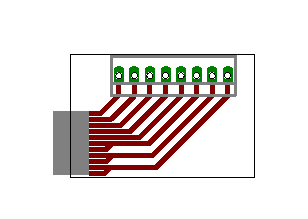
\includegraphics[width=\textwidth]{figures/expansion_board.pdf}
		\caption{Left leg extension PCB schematic}
		\label{fig:pcb1}
	\end{subfigure}
	\begin{subfigure}[b]{0.4\textwidth}
		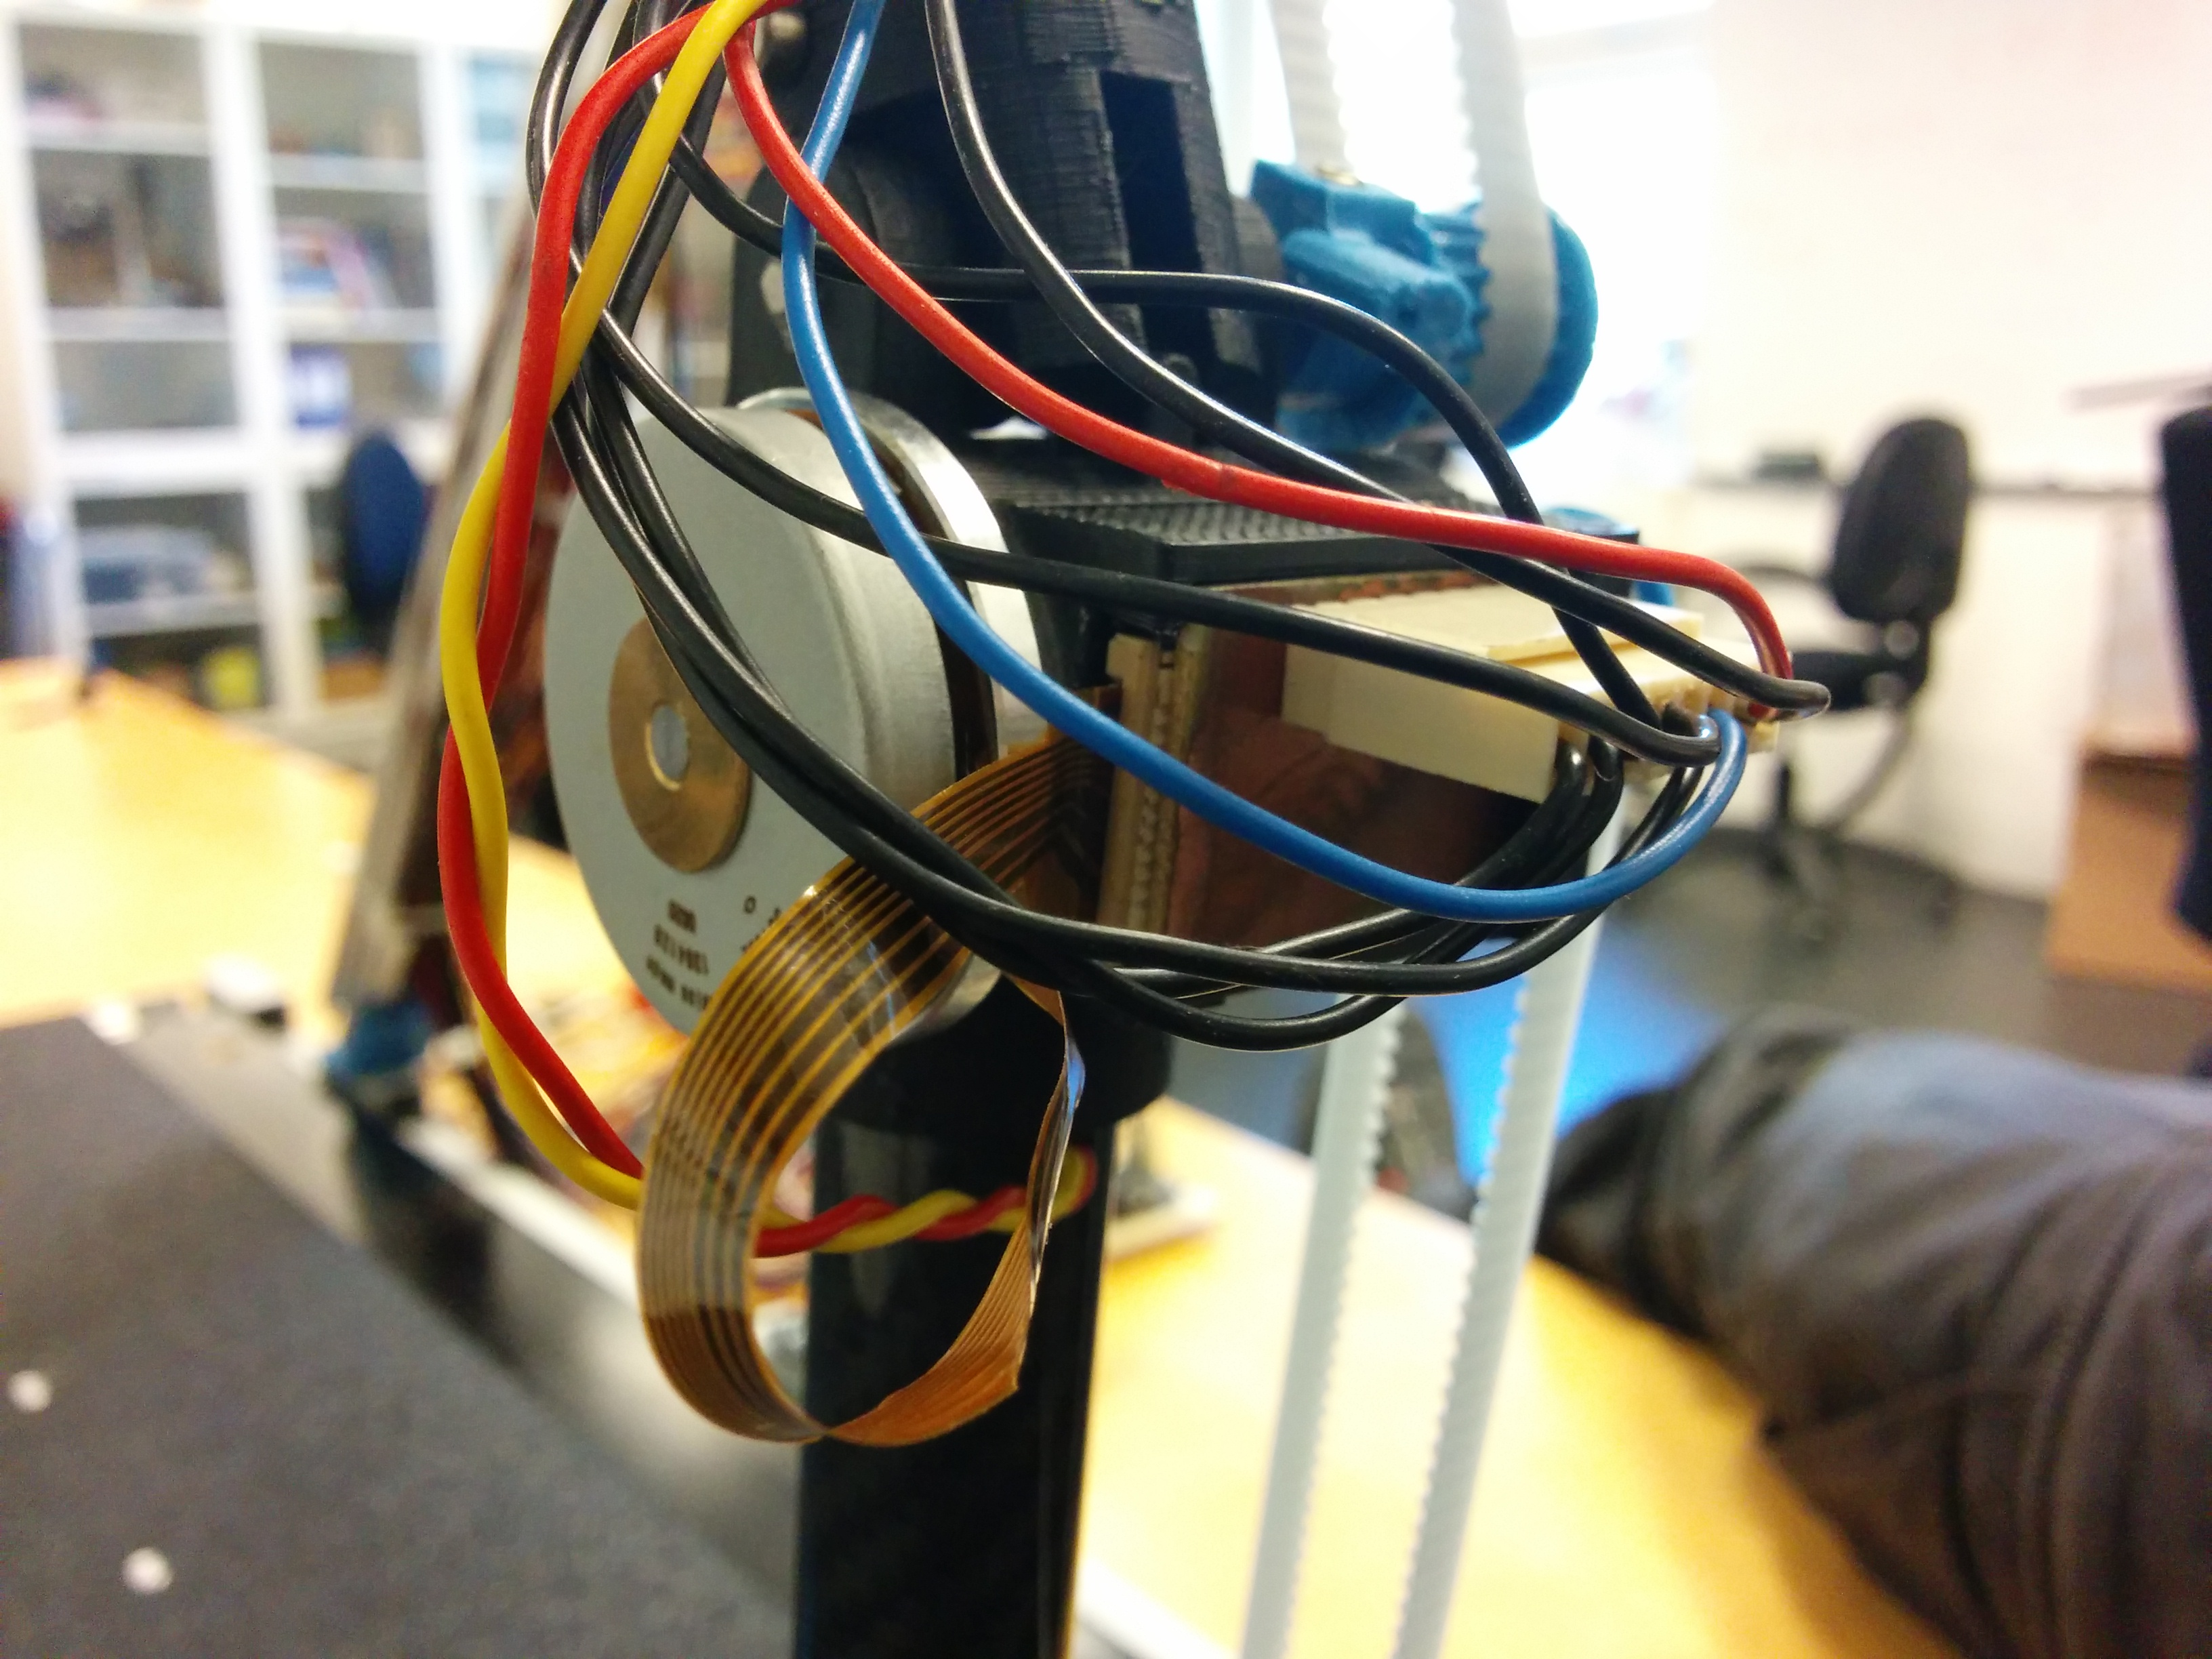
\includegraphics[width=\textwidth]{figures/photo_electronics_detail.jpg}
		\caption{Left leg extension PCB implemented}
		\label{fig:pcb2}
	\end{subfigure}
	\caption{Extension boards for motor control}
\end{figure}

New Molex connectors have been soldered to the original boards in order to implement these extensions, as shown in Figure \ref{fig:electronics2} within the final arrangement of the motor boards and the main processor board.
A distinctive color has been chosen for the wiring of each motor just to ease the task of arranging the final configuration.
Every motor board is labeled with the name of the joint it drives and matched to the appropriate address from the main processor by software, as explained in \ref{sub:ros_control_hardware_locokit_interface}.
This means that if a BLDC motor board is going to be changed, both its physical connection, label and internal address have to be changed accordingly.

\begin{figure}[h]
\centering
	\begin{subfigure}[b]{0.4\textwidth}
		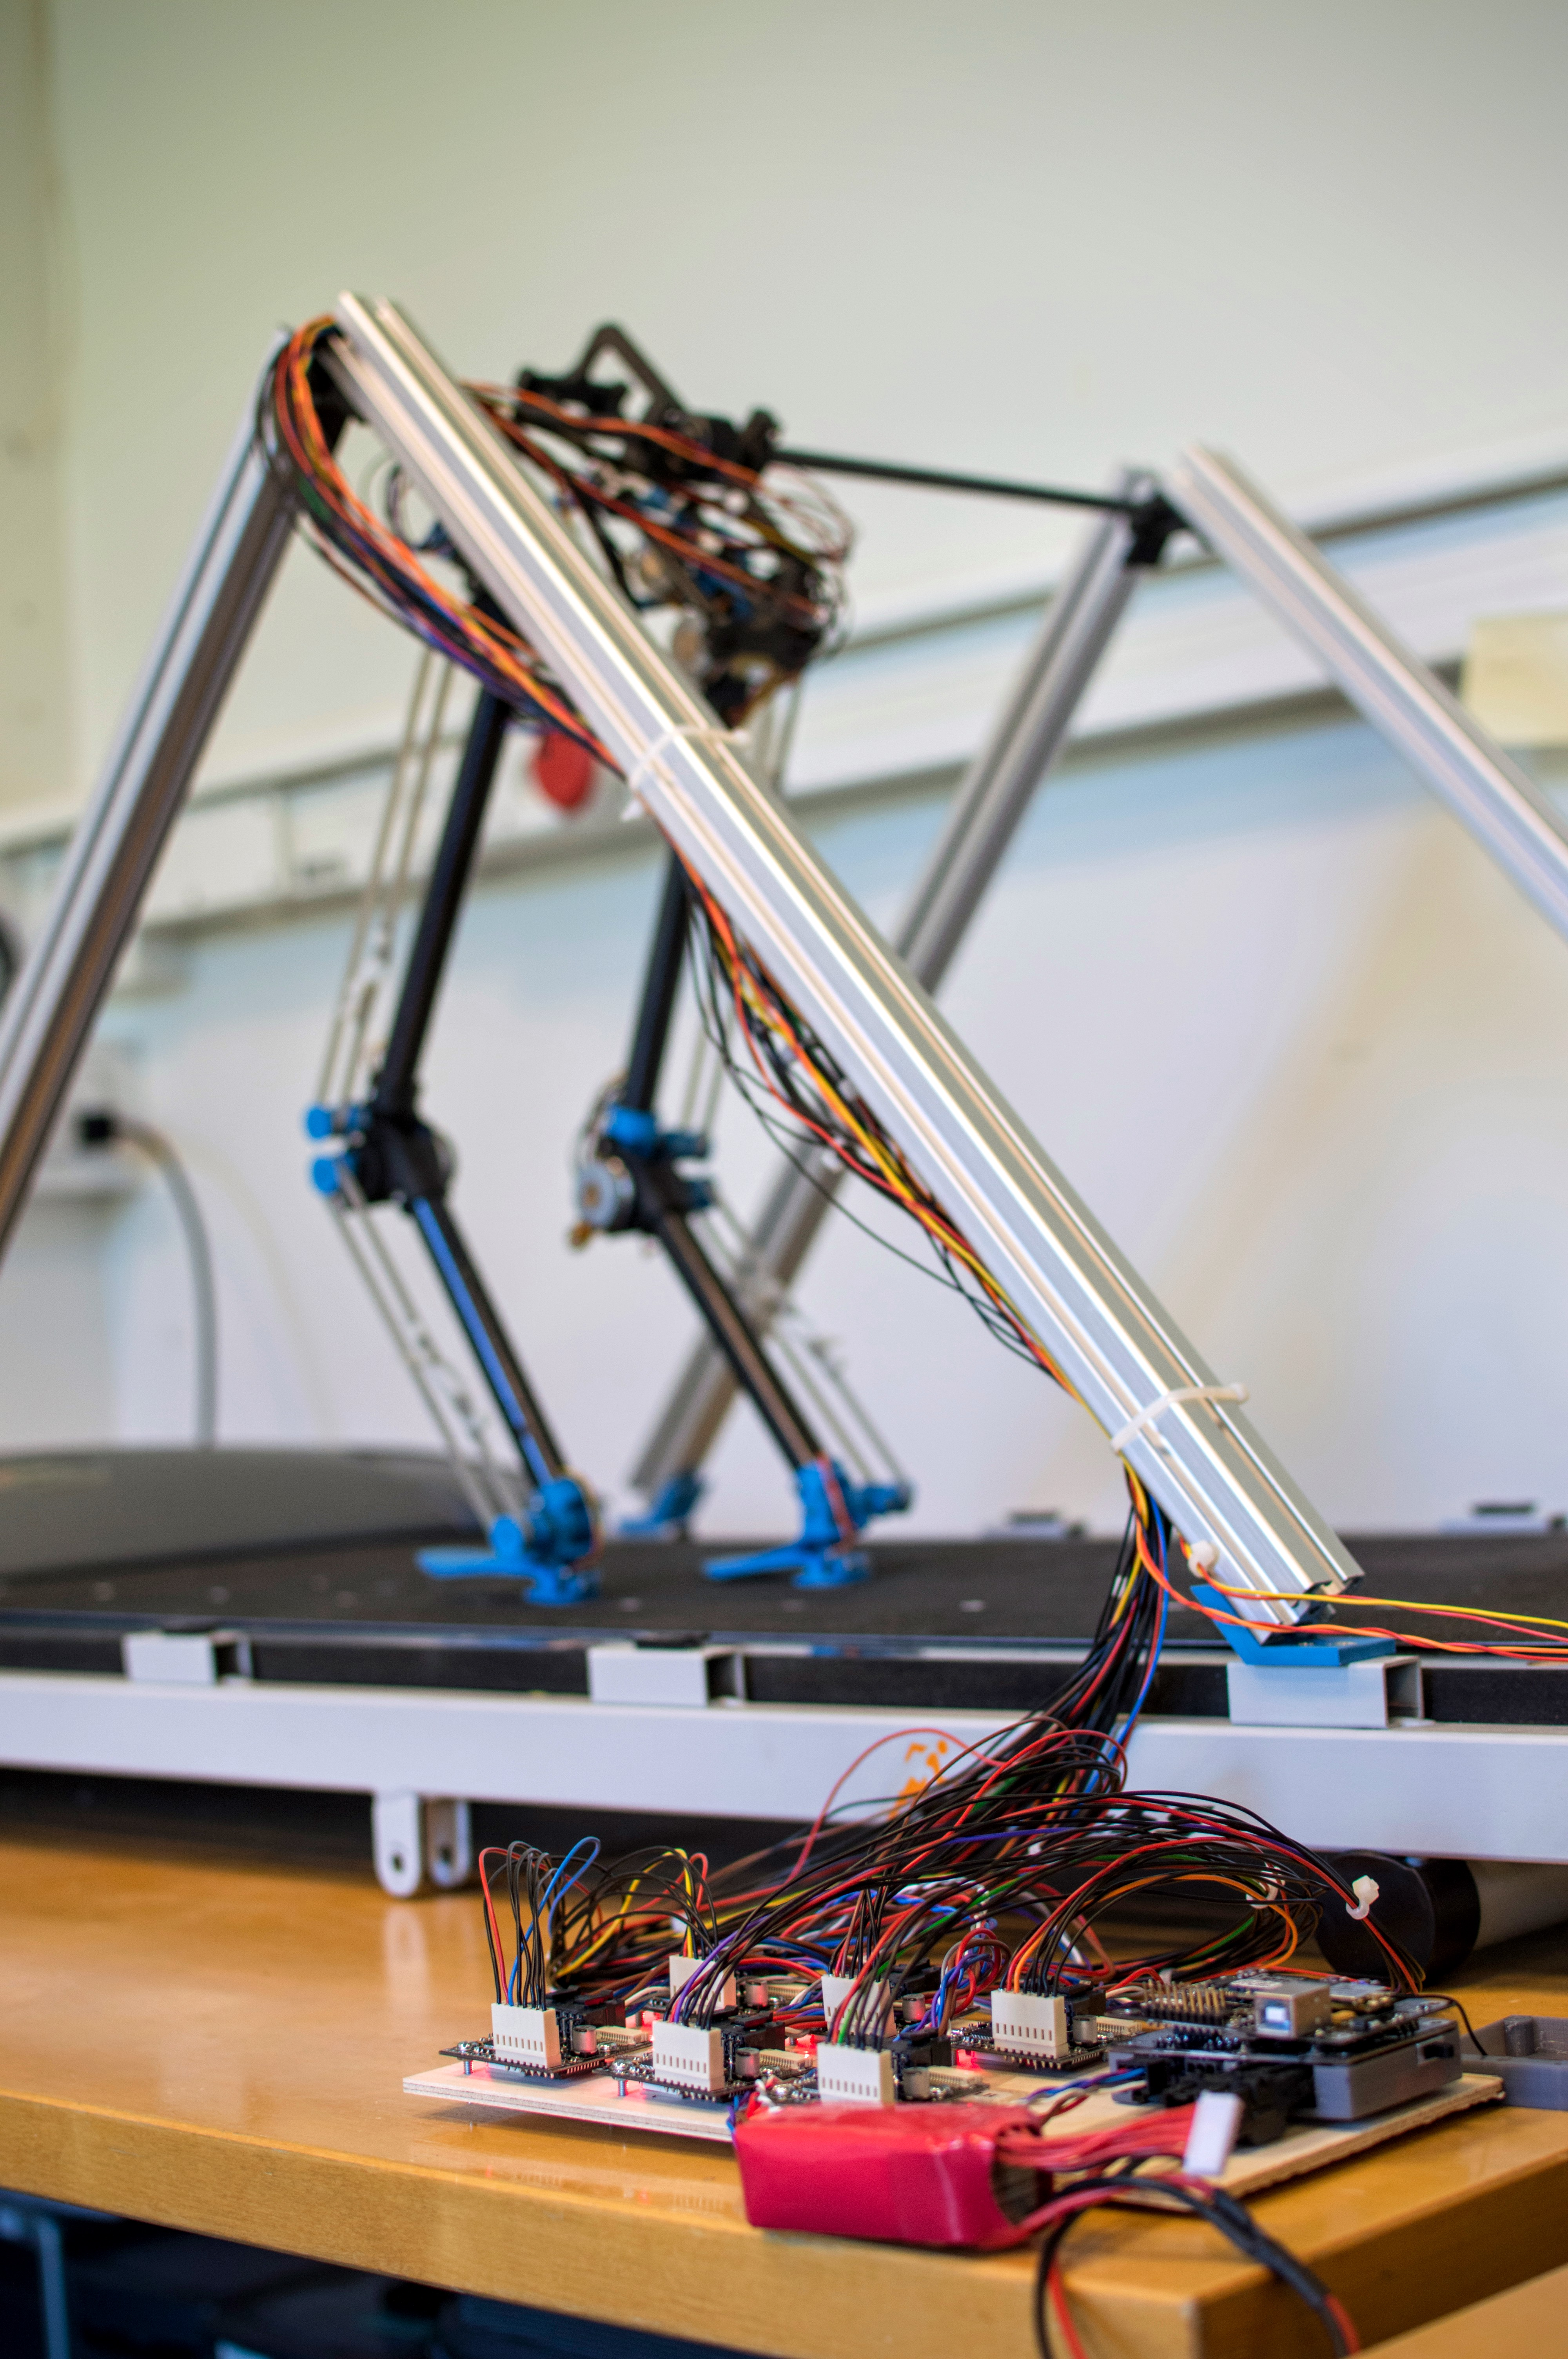
\includegraphics[width=\textwidth]{figures/photo_electronics_2.jpg}
		\caption{Wiring on the structure}
		\label{fig:electronics1}
	\end{subfigure}
	\begin{subfigure}[b]{0.4\textwidth}
		\includegraphics[width=\textwidth]{figures/photo_electronics.jpg}
		\caption{Electronics main board}
		\label{fig:electronics2}
	\end{subfigure}
	\caption{Final architecture of electronics}
\end{figure}

% subsubsection extension_pcbs (end)


% subsection electric_actuators (end)